% \iffalse meta-comment
%
% ontesting.dtx
% 22 January 2013
%
% This is version 1.1
%    It generates a test bed  (testsample.tex) for the sample shape, 
%       and an article (ontesting.pdf) on the tests.
%
% Generation of testsample.tex is with    
%    pdflatex makeshape.ins
% which contains   
%    \generate{\file{testsample.tex}
%                    {\from{ontesting.dtx}{testbed}}}
%
% Generation of ontesting.pdf is with
%    pdflatex ontesting.dtx
%
% The \OnlyDescription command is not used for this document.
%
% This is part of Silhouette 2.1
%
% ------------------------------------------------------------------
% \fi
%
% \iffalse
%^^A---------------------------------------------------------
%^^A        Preamble for documentation
%^^A---------------------------------------------------------
%<*driver>
\documentclass[10pt,a4paper]{ltxdoc}

\usepackage[T1]{fontenc}
\usepackage{lmodern}

\usepackage{hyperref}

\usepackage{makeshape}
\GetFileInfo{makeshape.sty}

\newcommand{\mnote}[1]
{\marginpar{\scriptsize \raggedright #1 }}

\EnableCrossrefs
\CodelineIndex
\RecordChanges

\begin{document}
\DocInput{ontesting.dtx}
\end{document}
%</driver>
% \fi
%
%^^A-------------------------------------------------------------------
%^^A      Change log...
%^^A-------------------------------------------------------------------
%^^A
%^^A 0.0 - 6 January 2013
%    \changes{0.0}{2013/01/06}{
%       Experimental - part of Silhouette 2.0.1.
%       Testing code is adopted from existing documents but improved.    
%       Monolithic testing code generation.
%       User documentation is incomplete. 
%    }
%^^A
%^^A 1.0 - 9 January 2013 (started 7 January)
%    \changes{1.0}{2013/01/09}{
%       \emph{Experimental phase complete.}
%       Testing code generation is embedded in the documentation.
%       Testing code is updated with improved tests.
%       Documentation on the role of the tests is completed.
%       File names are finalised. 
%    }
%^^A
%^^A 1.1 - 22 January 2013
%    \changes{1.1}{2013/01/22}{
%       Tidied up the structure and layout of the test code. 
%       The description of the tests is improved.
%       The report's title is changed.
%    }
%^^A
%^^A-------------------------------------------------------------------
%^^A     Check sums... 
%^^A-------------------------------------------------------------------
% 
%^^A no checksum required
%
% \CharacterTable
%  {Upper-case    \A\B\C\D\E\F\G\H\I\J\K\L\M\N\O\P\Q\R\S\T\U\V\W\X\Y\Z
%   Lower-case    \a\b\c\d\e\f\g\h\i\j\k\l\m\n\o\p\q\r\s\t\u\v\w\x\y\z
%   Digits        \0\1\2\3\4\5\6\7\8\9
%   Exclamation   \!     Double quote  \"     Hash (number) \#
%   Dollar        \$     Percent       \%     Ampersand     \&
%   Acute accent  \'     Left paren    \(     Right paren   \)
%   Asterisk      \*     Plus          \+     Comma         \,
%   Minus         \-     Point         \.     Solidus       \/
%   Colon         \:     Semicolon     \;     Less than     \<
%   Equals        \=     Greater than  \>     Question mark \?
%   Commercial at \@     Left bracket  \[     Backslash     \\
%   Right bracket \]     Circumflex    \^     Underscore    \_
%   Grave accent  \`     Left brace    \{     Vertical bar  \|
%   Right brace   \}     Tilde         \~}
%
%^^A===========================================================================
%^^A Start report body
%^^A===========================================================================
%
% \title{The {\sf makeshape} package\thanks{
%        This document is part of \textsf{makeshape}~\fileversion, dated~\filedate.}\\ 
% {\tt testshape.tex}\\A Document for Testing the Package and \\Custom Shapes}
%
% \author{Adrian P. Robson\thanks{\texttt{adrian.robson@nepsweb.co.uk}}}
% \date{22 January 2013}
%
% \maketitle
%
% \tableofcontents
%
%\section{Introduction}
%
% Here we discus the |testsample.tex| document 
% that is a test bed for the {\sf makeshape} package \cite{makeshape} 
% and its sample shape.
% The package is in |makeshape.sty| and the sample shape is defined in |sampleshape.tex|.
% The test bed can be usefully adapted to work with any PGF \cite{pgfMan} shape  
% developed with the {\sf makeshape} package. 
%
% There are 11 test PGF pictures in the |testsample.tex| document, 
% and we describe what each of these tests achieves, and what aspects are important for custom shapes.
%
%
%^^A#################################################################
%^^A# Test bed document - preamble - start
%^^A#################################################################
%\iffalse
%<*testbed>
%%--------------------------------------------------------
%%
%% This is a test bed for the makeshape package's 
%% sampleshape in sampleshape.tex
%%
%% It can be easily adapted for other shapes.
%%
%% 22 January 2013

\documentclass[10pt,a4paper]{article}

\usepackage{enumitem}
\usepackage{tikz}
\usetikzlibrary{backgrounds}
\usetikzlibrary{arrows}

%%-------------------------------------------------
%% file and shape being tested
\def\filename{sampleshape}   % file being tested
\input{\filename}            % It is a .tex 
%%\usepackage{\filename}     % It is a .sty
\def\testshape{sample}       % shape being tested
%%-------------------------------------------------

%%--------------------------------------------------------
%%    Utility macros
%%--------------------------------------------------------

%% \spot{x}{y}
\newcommand{\spot}[2]{
   \draw[help lines,red] (#1,#2) circle (1pt);
}

%% \markOrig
\def\mrksz{4pt}
\def\mrkcol{yellow}
\newcommand{\markOrig}{
   \draw[help lines,\mrkcol] (0,0) circle (\mrksz);
   \draw[help lines,\mrkcol] (-\mrksz,0) -- (\mrksz,0);
   \draw[help lines,\mrkcol] (0,-\mrksz) -- (0,\mrksz);
}

%% \markOrigC{colour}
\def\mrksz{4pt}
\newcommand{\markOrigC}[1]{
   \draw[help lines,#1] (0,0) circle (\mrksz);
   \draw[help lines,#1] (-\mrksz,0) -- (\mrksz,0);
   \draw[help lines,#1] (0,-\mrksz) -- (0,\mrksz);
}

%% Anchors ...
%%    \***{node}{size}{colour}

\def\centeranchor#1#2#3{
   \draw[help lines,#3] (#1.center) circle (#2);
}

\def\textanchor#1#2#3{
   \draw[help lines,#3] (#1.text) circle (#2);
}

\def\cardinalanchors#1#2#3{
   \draw[help lines,#3] (#1.north) circle (#2);
   \draw[help lines,#3] (#1.west) circle (#2);
   \draw[help lines,#3] (#1.south) circle (#2);
   \draw[help lines,#3] (#1.east) circle (#2);
}

\def\corneranchors#1#2#3{
   \draw[help lines,#3] (#1.north west) circle (#2);
   \draw[help lines,#3] (#1.south west) circle (#2);
   \draw[help lines,#3] (#1.south east) circle (#2);
   \draw[help lines,#3] (#1.north east) circle (#2);
}

\def\allanchors#1#2#3{
   \corneranchors{#1}{#2}{#3}
   \cardinalanchors{#1}{#2}{#3}
}

%%--------------------------------------------------------

\title{The {\sf makeshape} package\\
       Shape Test Bed
       \vspace{-3ex} }
\author{}
\date{
\begin{tabular}{rl}
       File  & {\tt \filename}\\
       Shape & {\tt \testshape} 
\end{tabular}
\\[2ex]
\today}

\begin{document}

\maketitle

%</testbed>
%\fi
%^^A#################################################################
%^^A# Test bed document - preamble - end
%^^A#################################################################
%
% \section{The Tests}
%
% \subsection{Basic Shape}
%
%  This section shows the shape with its default size and separation options.
%  Cardinal anchor points are show in red; the centre anchor in blue; 
%  and the text anchor in green.
%  The green lines show the the text box size. 
%
%  It tests the package's management of the text box, the text and centre anchors,
%  and the shape's cardinal anchors.  
% \emph{Check that the background path is correct, 
%       and that the anchors are in the correct positions.}
%
%^^A#################################################################
%^^A# Test bed document - basic shape tests - start
%^^A#################################################################
%\iffalse
%<*testbed>
%%--------------------------------------------------------
\section*{Basic Shape}

\begin{center}
\begin{tikzpicture}

\node at (0,0)
   [\testshape, draw
   ] (test) {\verb|x         x|} ;

\allanchors{test}{2pt}{red}
\textanchor{test}{2pt}{green}
\draw[help lines,green] (test.text) -- ++(7pt,0);
\draw[help lines,green] (test.text) -- ++(0,5pt);
\centeranchor{test}{2pt}{blue}

%% mark the anchors with arrows from enclosing rectangle
\node at (0,0)
   [rectangle, red,
    minimum width=4cm,
    minimum height=2cm
   ] (outer) {} ;
\begin{scope}[>=latex']
\draw[->,help lines,red] (outer.north) -- (test.north);
\draw[->,help lines,red] (outer.east) -- (test.east);
\draw[->,help lines,red] (outer.south) -- (test.south);
\draw[->,help lines,red] (outer.west) -- (test.west);
\draw[->,help lines,red] (outer.north east) -- (test.north east);
\draw[->,help lines,red] (outer.south east) -- (test.south east);
\draw[->,help lines,red] (outer.south west) -- (test.south west);
\draw[->,help lines,red] (outer.north west) -- (test.north west);
\end{scope}

\begin{scope}[on background layer]
\node at (4cm,0)
   [rectangle, draw
   ] (rectRmin) {\verb|x         x|};

\node at (0,-1.7cm)
   [rectangle, draw
   ] (rectBmin) {\verb|x         x|};

\draw[help lines,green] (rectRmin.north west) -- ++(-4.5cm,0);
\draw[help lines,green] (rectRmin.south west) -- ++(-4.5cm,0);
\draw[help lines,green] (rectBmin.north west) -- ++(0,2.3cm);
\draw[help lines,green] (rectBmin.north east) -- ++(0,2.3cm);
\markOrig
\end{scope}

\end{tikzpicture}

\end{center}

%</testbed>
%\fi
%^^A#################################################################
%^^A# Test bed document - basic shape tests - end
%^^A#################################################################
%
% \subsection{Minimum Dimensions}
%
% This tests support for minimum width and height keys.
% Yellow lines mark the required sizes and centres, and  
% green lines show the text box location.
% Cardinal anchors are shown in red. 
%
% \emph{Check that the background path has scaled properly to the correct dimensions;
% and the anchors are in the right places.}
%
%^^A#################################################################
%^^A# Test bed document - minimum dimension tests - start
%^^A#################################################################
%\iffalse
%<*testbed>
\vfill
%%--------------------------------------------------------
\section*{Minimum Dimensions}

\def\minh{30pt}
\def\minw{80pt}

{\tt minimum width = \minw}\\
{\tt minimum height = \minh}

\begin{center}
\begin{tikzpicture}

%% The test shape
\node at (0,0)
   [\testshape, draw,
    minimum width=\minw,
    minimum height=\minh,
   ] (test) {\verb|x   x|} ;

\allanchors{test}{1pt}{red}

%% Guide lines
\begin{scope}[on background layer]
\node at (4.5cm+\minw,0)
   [rectangle, draw
   ] (rectRmin) {\verb|x   x|};

\node at (1.5cm+\minw,0)
   [rectangle, draw,
    minimum width=\minw,
    minimum height=\minh
   ] (rectR) {\verb|x   x|};

\node at (0,-1cm-\minh)
   [rectangle, draw,
    minimum width=\minw,
    minimum height=\minh
   ] (rectB) {\verb|x   x|};

\node at (0,-2.5cm-\minh)
   [rectangle, draw,
   ] (rectBmin) {\verb|x   x|};

\markOrig
\draw[help lines,yellow] (rectR.north west) -- ++(-1.7cm-\minw,0);
\draw[help lines,yellow] (rectR.south west) -- ++(-1.7cm-\minw,0);
\draw[help lines,yellow] (rectR.west) -- ++(-1.7cm-\minw,0);
\draw[help lines,yellow] (rectR.west) -- ++(\minw+0.2cm,0);
\draw[help lines,yellow] (rectB.north west) -- ++(0,1.2cm+\minh);
\draw[help lines,yellow] (rectB.north east) -- ++(0,1.2cm+\minh);
\draw[help lines,yellow] (rectB.north) -- ++(0,1.2cm+\minh);
\draw[help lines,yellow] (rectB.north) -- ++(0,-\minh-0.2cm);

\draw[help lines,green] (rectRmin.north west) -- ++(-4.6cm-\minw,0);
\draw[help lines,green] (rectBmin.north west) -- ++(0,2.6cm+\minh);
\end{scope}

\end{tikzpicture}
\end{center}
\vfill

%</testbed>
%\fi
%^^A#################################################################
%^^A# Test bed document - minimum dimension tests - end
%^^A#################################################################
%
% \subsection{Inner Separation}
%
% This tests support for the inner separation keys.
% Inner separation is handled by the package and is included in 
% the corrected text box. 
% Green lines show the basic text box location, and
% blue lines show the corrected text box location.
% Cardinal anchors are shown in red. 
%
% \emph{Check that the shape has scaled properly under the influence of the two keys;
% and the anchors are in the right places.}
%
%^^A#################################################################
%^^A# Test bed document - inner separation tests - start
%^^A#################################################################
%\iffalse
%<*testbed>
\newpage
%%--------------------------------------------------------
\section*{Inner Separation}

\def\insepx{20pt}
\def\insepy{10pt}

{\tt inner x seperation = \insepx}\\
{\tt inner y seperation = \insepy}

\begin{center}
\begin{tikzpicture}

%% The test shape
\node at (0,0)
   [\testshape, draw,
    inner xsep=\insepx, inner ysep=\insepy
   ] (test) {\verb|x   x|} ;

\allanchors{test}{1pt}{red}

%% Guide lines
\begin{scope}[on background layer]
\markOrig

\node at (2.5cm,0)
   [rectangle, draw 
   ] (rectRmin) {\verb|x   x|};

\node at (0,-1.5cm)
   [rectangle, draw 
   ] (rectBmin) {\verb|x   x|};

\node at (4cm,0)
   [rectangle, draw, 
    inner ysep=\insepy
   ] (rectRwithSep) {\verb|x   x|};

\node at (0,-2.2cm)
   [rectangle, draw, 
    inner xsep=\insepx
   ] (rectBwithSep) {\verb|x   x|};

\draw[help lines,green] (rectRmin.north west) -- ++(-3.4cm,0);
\draw[help lines,green] (rectBmin.north west) -- ++(0,2cm);
\draw[help lines,blue] (rectRwithSep.north west) -- ++(-4.9cm,0);
\draw[help lines,blue] (rectBwithSep.north west) -- ++(0,2.7cm);
\end{scope}

\end{tikzpicture}
\end{center}

%</testbed>
%\fi
%^^A#################################################################
%^^A# Test bed document - inner separation tests - end
%^^A#################################################################
%
% \subsection{Outer Separation}
%
% This section tests the outer separation keys.
% The actual shape is drawn in black. 
% To shown the boundary of the outer separation surface, 
% the shape is expanded and drawn in green. 
% Anchors, which should be on this surface are displayed in red. 
%
% \emph{Check that the expanded green shape is well formed, 
% and that the anchors are in the correct place.}
%
%^^A#################################################################
%^^A# Test bed document - outer separation tests - start
%^^A#################################################################
%\iffalse
%<*testbed>
%%--------------------------------------------------------
\section*{Outer Separation}

\def\minh{20pt}
\def\minw{60pt}
\def\outerx{20pt}
\def\outery{10pt}

{\tt outer x separation = \outerx}\\
{\tt outer y separation = \outery}

\begin{center}
\begin{tikzpicture}

\markOrig

%% the shape with outer separation
\node at (0,0)
   [\testshape, draw, 
    minimum width=\minw,
    minimum height=\minh,
    outer xsep=\outerx, outer ysep=\outery
   ] (test) {\verb|x   x|} ;

%% shape expanded to outer separation boundary
\node at (0,0)
   [\testshape, draw, help lines, green,
    minimum width=\minw+2*\outerx,
    minimum height=\minh+2*\outery,
   ] (bigger) {} ;

%% mark the anchors with arrows from enclosing rectangle
\node at (0,0)
   [rectangle,
    minimum width=\minw+1cm, 
    minimum height=\minh+1cm,
    outer xsep=\outerx, outer ysep=\outery
   ] (outer) {} ;

\begin{scope}[>=latex']
\draw[->,help lines,red] (outer.north) -- (test.north);
\draw[->,help lines,red] (outer.east) -- (test.east);
\draw[->,help lines,red] (outer.south) -- (test.south);
\draw[->,help lines,red] (outer.west) -- (test.west);
\draw[->,help lines,red] (outer.north east) -- (test.north east);
\draw[->,help lines,red] (outer.south east) -- (test.south east);
\draw[->,help lines,red] (outer.south west) -- (test.south west);
\draw[->,help lines,red] (outer.north west) -- (test.north west);
\end{scope}

%% mark anchors with circles
\allanchors{test}{2pt}{red}

%% mark text and centre anchors
\textanchor{test}{2pt}{green}
\draw[help lines,green] (test.text) -- ++(7pt,0);
\draw[help lines,green] (test.text) -- ++(0,5pt);
\centeranchor{test}{2pt}{blue}

\end{tikzpicture}
\end{center}

%</testbed>
%\fi
%^^A#################################################################
%^^A# Test bed document - outer separation tests - end
%^^A#################################################################
%
% \subsection{Anchorborder}
%
% There are three tests that are applied to verify the behaviour of 
% the package's |\anchorborder|, and the shape's anchor path.
%
%\iffalse
%<*testbed>
%%--------------------------------------------------------
\section*{Anchorborder }

%</testbed>
%\fi
%
% \subsubsection{\texorpdfstring{External Points with Outer Separation and\\
%                                Minimum Dimensions}
%                               {External Points with Outer Separation and
%                                Minimum Dimensions}}
% 
%  This tests the connection of an external point to the shape's surface.
%  It exercises outer separation and minimum dimensions.
%  The black surface is the shape without any separation, 
%  and the outer green surface is where the outer separation surface should be.
%  \emph{Check that the black arrows touch the outer green surface; 
%  and that the green shape is correct.}
%
%^^A#################################################################
%^^A# Test bed document - external points with outer separation and
%^^A#                     minimum dimensions tests - start
%^^A#################################################################
%\iffalse
%<*testbed>
%%--------------------------------------------------------
\subsection*{External Points with Outer Separation and\\Minimum Dimensions}

\def\width{2cm}
\def\height{1cm}
\def\testouter{10pt}

{\tt outer sep = \testouter}\\
{\tt minimum height = \height}\\
{\tt minimum width = \width}

\begin{center}
\begin{tikzpicture}

\markOrig

%% The test shape
\node at (0,0) [\testshape, draw, font={\sf \small},
                minimum width=\width,
                minimum height=\height,
                outer sep=\testouter
               ] (test) {Test};

%% green path where anchors should be
\node at (0,0) [\testshape, draw, help lines, green, 
                minimum width=\width+2*\testouter,
                minimum height=\height+2*\testouter,
               ] (bigger) {} ;

\def\n{20}
\def\radius{3cm}
\draw[dotted] (0,0) circle (\radius);
\foreach \s in {1,...,\n}
{
  \draw[->, >=latex']  ({360/\n * (\s - 1)}:\radius) -- (test);
}
\end{tikzpicture}
\end{center}

%</testbed>
%\fi
%^^A#################################################################
%^^A# Test bed document - external points with outer separation and 
%^^A#                     minimum dimensions tests - end
%^^A#################################################################
%
% \subsubsection{Internal Points with Minimum Dimensions}
% 
%  This tests the connection of an internal point to the shape's surface.
%  It uses minimum dimensions.
%  \emph{Check that the red arrows touch the outer black surface, 
%    and that the black shape is correct.}
%
%^^A#################################################################
%^^A# Test bed document - internal points with minimum dimensions
%^^A#                     tests - start
%^^A#################################################################
%\iffalse
%<*testbed>
%%--------------------------------------------------------
\subsection*{Internal Points with Minimum Dimensions}

\def\width{3cm}
\def\height{3cm}

{\tt minimum height = \height}\\
{\tt minimum width = \width}

\vspace{-3ex}
\begin{center}
\begin{tikzpicture}

\markOrig

%% The test shape
\node at (0,0) [\testshape, draw, font={\sf \small},
                minimum width=\width,
                minimum height=\height,
               ] (test) {};

\def\n{20}
\def\radius{1cm}
\draw[dotted] (0,0) circle (\radius);
\foreach \s in {1,...,\n}
{
  \draw[->, >=latex', red]  ({360/\n * (\s - 1)}:\radius) -- (test);
}
\end{tikzpicture}
\end{center}

%</testbed>
%\fi
%^^A#################################################################
%^^A# Test bed document - internal points with minimum dimensions
%^^A#                     tests - end
%^^A#################################################################

% \subsubsection{Angles with Outer Separation and Minimum Dimensions}
%
% This tests the `connect a line at an angle' feature. 
% Different x and y outer separations and minimum dimensions are used.
% The black surface is the shape without any separation, 
% and the outer red surface is where the outer separation surface should be.
% \emph{Check that the blue dots are on the outer red surface, 
%  and that the red shape is correct.}
%
%^^A#################################################################
%^^A# Test bed document - angles with outer separation and minimum
%^^A#                     dimensions tests - start
%^^A#################################################################
%\iffalse
%<*testbed>
%%--------------------------------------------------------
\subsection*{Angles with Outer Separation and Minimum Dimensions}

\def\angle{120}
\def\width{2cm}
\def\height{1cm}
\def\testouterx{20pt}
\def\testoutery{10pt}

Marked angle = \angle\\
{\tt outer xsep = \testouterx}\\
{\tt outer ysep = \testoutery}\\
{\tt minimum height = \height}\\
{\tt minimum width = \width}

\vspace{-5ex}
\begin{center}
\begin{tikzpicture}

\markOrig

%% red path where anchors should be ?
\node at (0,0) [\testshape, draw, help lines, red, 
                minimum width=\width+2*\testouterx,
                minimum height=\height+2*\testoutery,
               ] (bigger) {};

\node at (0,0) [\testshape, draw,
                minimum width=\width,
                minimum height=\height,
                outer xsep=\testouterx,
                outer ysep=\testoutery
               ] (test) {};

\foreach \angle in {0,5,...,355} {
  \fill[blue] (test.\angle) circle[radius=1pt];
}

%% single angle test
\def\angle{120}
\draw [help lines] (test.center) -- ++(\angle:1.5cm);
\draw[green] (test.\angle) circle[radius=2pt];
\draw[green] (test.\angle) -- ++(3pt,3pt);
\draw[green] (test.\angle) -- ++(-3pt,-3pt);
\draw[green] (test.\angle) -- ++(-3pt,3pt);
\draw[green] (test.\angle) -- ++(3pt,-3pt);

\end{tikzpicture}
\end{center}

%</testbed>
%\fi
%^^A#################################################################
%^^A# Test bed document - angles with outer separation and minimum
%^^A#                     dimensions tests - end
%^^A#################################################################
%
% \subsection{Simple Node Connections}
%
%  This tests simple node connection. 
%  \emph{Check that the centre shape is connect to the surrounding eight shapes.} 
%
%^^A#################################################################
%^^A# Test bed document - simple node connections tests - start
%^^A#################################################################
%\iffalse
%<*testbed>
%%--------------------------------------------------------
\section*{Simple Node Connections}

\begin{center}
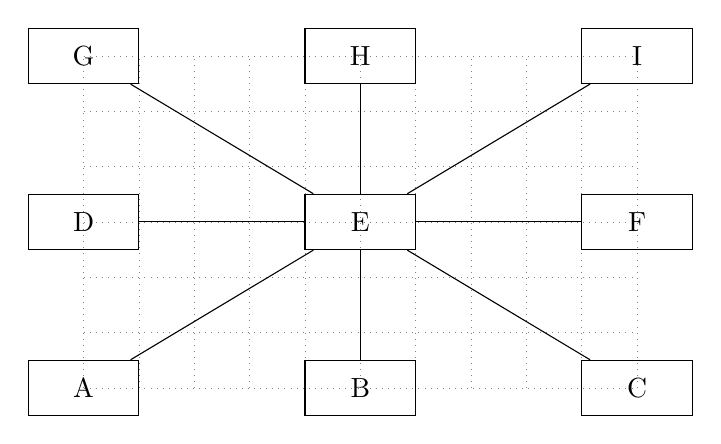
\begin{tikzpicture}
\def\ra{0} \def\rb{60pt} \def\rc{120pt}
\def\ca{0} \def\cb{100pt} \def\cc{200pt}

\draw[help lines,step=20pt,dotted] (0pt,0pt) grid (\cc,\rc);

\tikzset{node style/.style={ minimum width=40pt,minimum height=20pt}}

\markOrig

\node at (\ca,\ra) [draw, \testshape, node style] (A) {A};
\node at (\cb,\ra) [draw, \testshape, node style] (B) {B};
\node at (\cc,\ra) [draw, \testshape, node style] (C) {C};
%%
\node at (\ca,\rb) [draw, \testshape, node style] (D) {D};
\node at (\cb,\rb) [draw, \testshape, node style] (E) {E};
\node at (\cc,\rb) [draw, \testshape, node style] (F) {F};
%%
\node at (\ca,\rc) [draw, \testshape, node style] (G) {G};
\node at (\cb,\rc) [draw, \testshape, node style] (H) {H};
\node at (\cc,\rc) [draw, \testshape, node style] (I) {I};

\draw (E) -- (F);
\draw (E) -- (D);
\draw (E) -- (B);
\draw (E) -- (H);
\draw (E) -- (G);
\draw (E) -- (A);
\draw (E) -- (I);
\draw (E) -- (C);

\end{tikzpicture}
\end{center}

%</testbed>
%\fi
%^^A#################################################################
%^^A# Test bed document - simple node connections tests - end
%^^A#################################################################
%
% \subsection{Scaling}
%
%   This is a simple scaling test that uses minimum dimensions to draw 
%   the shape at three sizes. 
%   There are guide lines showing dimensions for each size.
%   \emph{Check that all of the shapes are correct.} 
%
%^^A#################################################################
%^^A# Test bed document - scaling tests - start
%^^A#################################################################
%\iffalse
%<*testbed>
%%--------------------------------------------------------
\section*{Scaling}

\def\minh{20pt}
\def\minw{80pt}
\def\exd{5pt}

\begin{center}
\begin{tikzpicture}

\node at (0,0)
   [\testshape, draw, 
    minimum width=\minw,
    minimum height=\minh,
   ] (test1) {} ;

\node at (0,0)
   [\testshape, draw, blue,
    minimum width=\minw+1cm,
    minimum height=\minh+1cm,
   ] (test2) {} ;

\node at (0,0)
   [\testshape, draw, red,
    minimum width=\minw+2cm,
    minimum height=\minh+2cm,
   ] (test3) {} ;

\def\tgridA#1#2{
\draw[help lines] ({0.5*(\minw+#1)+\exd},{0.5*(\minh+#1)}) -- ({-0.5*(\minw+#1)-\exd},{0.5*(\minh+#1)});
\draw[help lines] ({0.5*(\minw+#1)+\exd},{-0.5*(\minh+#1)}) -- ({-0.5*(\minw+#1)-\exd},{-0.5*(\minh+#1)});
\draw[help lines] ({0.5*(\minw+#1)},{0.5*(\minh+#1)+\exd}) -- ({0.5*(\minw+#1)},{-0.5*(\minh+#1)-\exd});
\draw[help lines] ({-0.5*(\minw+#1)},{0.5*(\minh+#1)+\exd}) -- ({-0.5*(\minw+#1)},{-0.5*(\minh+#1)-\exd});
}

\begin{scope}[on background layer]
\tgridA{0pt}{0pt}
\tgridA{1cm}{1cm}
\tgridA{2cm}{2cm}
\markOrig
\end{scope}

\end{tikzpicture}
\end{center}

%</testbed>
%\fi
%^^A#################################################################
%^^A# Test bed document - scaling tests - end
%^^A#################################################################
%
%
% \subsection{Package Tests}
%
%^^A#################################################################
%^^A# Test bed document - package tests peamble - start
%^^A#################################################################
%\iffalse
%<*testbed>
%%--------------------------------------------------------
\section*{Package Tests}

%</testbed>
%\fi
%^^A#################################################################
%^^A# Test bed document - package tests preamble- end
%^^A#################################################################
%
% \subsubsection{Text Alignment and the Text Box}
%
%  This verifies the operation of the text box macros.
%  All combinations of test ascenders and descenders are used.
%  It tests the package's management of the text box and the text and centre anchors.
% The left hand shapes are standard text boxes.
%
%  \emph{ 
%  Check the shape's text boxes align with the standard boxes.
%  Also that the blue centre anchor is at the yellow origin; 
%  and the green text anchor is in the correct place.
%  Finally, the red cardinal anchors should be suitably located on the shapes boundary.  }
%
%^^A#################################################################
%^^A# Test bed document - text alignment and 
%^^A#                     the text box tests - start
%^^A#################################################################
%\iffalse
%<*testbed>
%%--------------------------------------------------------
\subsection*{Text Alignment and the Text Box}

\begin{center}
\begin{tikzpicture}

\node at (0,0) 
     [\testshape, draw
     ] (test1) {\verb|x         x|} ;

\node[ \testshape, draw,
       below of=test1,
       node distance=1cm
     ] (test2) {\verb|x        dx|} ;

\node[ \testshape, draw,
       below of=test2, node distance=1cm
     ] (test3) {\verb|xp        x|} ;

\node[ \testshape, draw,
       below of=test3, node distance=1cm
     ] (test4) {\verb|xp       dx|} ;

\allanchors{test1}{1pt}{red}
\corneranchors{test2}{1pt}{red}
\corneranchors{test3}{1pt}{red}
\corneranchors{test4}{1pt}{red}
\centeranchor{test1}{2pt}{blue}
\centeranchor{test2}{2pt}{blue}
\centeranchor{test3}{2pt}{blue}
\centeranchor{test4}{2pt}{blue}
\textanchor{test1}{1pt}{green}
\draw[help lines,green] (test1.text) -- ++(7pt,0);
\draw[help lines,green] (test1.text) -- ++(0,5pt);
\textanchor{test2}{1pt}{green}
\textanchor{test3}{1pt}{green}
\textanchor{test4}{1pt}{green}

\begin{scope}[on background layer]

\markOrig

\node at(4cm,0) [ rectangle, draw
     ] (ref1) {\verb|x         x|} ;
\draw[green] (ref1.north west) -- ++(-5cm,0);
\draw[green] (ref1.south west) -- ++(-5cm,0);

\node[rectangle, draw,
      below of=ref1, node distance=1cm
     ] (ref2) {\verb|x        dx|} ;
\draw[green] (ref2.north west) -- ++(-5cm,0);
\draw[green] (ref2.south west) -- ++(-5cm,0);

\node[rectangle, draw,
      below of=ref2, node distance=1cm
     ] (ref3) {\verb|xp        x|} ;
\draw[green] (ref3.north west) -- ++(-5cm,0);
\draw[green] (ref3.south west) -- ++(-5cm,0);

\node[rectangle, draw,
      below of=ref3, node distance=1cm
     ] (ref4) {\verb|xp       dx|} ;
\draw[green] (ref4.north west) -- ++(-5cm,0);
\draw[green] (ref4.south west) -- ++(-5cm,0);

\end{scope}

\end{tikzpicture}
\end{center}

%</testbed>
%\fi
%^^A#################################################################
%^^A# Test bed document - text alignment and 
%^^A#                     the text box tests - end
%^^A#################################################################
%
% \subsubsection{Inner, Outer and Angle for Shape Off Origin}
% 
% This is a test for the correct operation of the package's |\anchorborder| 
% with off-origin shapes.
% In particular, its use of the |\pgf@relevantforpicturesizefalse|
% and |\pgftransformreset| commands.
%
% \emph{Check that the outer box `closely' contains the picture, 
% and that the green arrows and points are on the shape's boundary.}
%
%^^A#################################################################
%^^A# Test bed document - inner, outer and angle for shape off 
%^^A#                     origin tests - start
%^^A#################################################################
%\iffalse
%<*testbed>
%%--------------------------------------------------------
\subsection*{Inner, Outer and Angle for Shape Off Origin}

The box should closely contain picture if {\tt anchorborder} is working correctly.
\bigskip

\begin{center}
\begin{tikzpicture}[framed]

\markOrigC{black}
\draw (2pt,0) node[anchor=west]{\tt \tiny origin};

%% The test shape
\node at (70pt,40pt)
   [\testshape, draw,
    red, minimum width=60pt, minimum height=40pt
   ] (node) {};

%% outer test line
\path (node);
\pgfgetlastxy{\macrox}{\macroy}
\coordinate (Xout) at (\macrox+20pt,\macroy+40pt);

\draw (Xout) circle(3pt);
\draw [help lines] (node.center) -- (Xout);
\draw [->, >=latex',green] (Xout) -- (node); % <<<

%% inner test line
\path (node);
\pgfgetlastxy{\macrox}{\macroy}
\coordinate (Xin) at (\macrox-5pt,\macroy-5pt);

\draw (Xin) circle(3pt);
\draw [help lines,shorten >=-1cm] (node.center) -- (Xin);
\draw [->, >=latex',green] (Xin) -- (node); % <<<

%% test angle
\def\angle{120}
\draw [help lines] (node.center) -- ++(\angle:1.5cm);
\draw[green] (node.\angle) circle[radius=2pt]; % <<<

\end{tikzpicture}
\end{center}

%</testbed>
%\fi
%^^A#################################################################
%^^A# Test bed document - inner, outer and angle for shape off 
%^^A#                     origin tests - end
%^^A#################################################################
%
%^^A#################################################################
%^^A# Test bed document - epilogue - start
%^^A#################################################################
%\iffalse
%<*testbed>
\end{document}
%</testbed>
%\fi
%^^A#################################################################
%^^A# Test bed document - epilogue - end
%^^A#################################################################
%
% \section{Reuse}
% 
% The |testsample.tex| file can be adapted to test other shapes developed using
% the {\sf makeshape} package. Find the following section:
% 
% \begin{verbatim}
% %%-------------------------------------------------
% %% file and shape being tested
% \def\filename{sampleshape}   % file being tested
% \input{\filename}            % It is a .tex 
% %%\usepackage{\filename}     % It is a .sty
% \def\testshape{sample}       % shape being tested
% %%-------------------------------------------------
% \end{verbatim}
% Then change |sampleshape| to the new file name, and |sample| to the particular shape's name.
% Choose |\input| or |\usepackage| dependinmg on the file type.
%
% The report's ending `Package Test' section can be deleted, and additional shape specific tests added. 
% The file's {\sf makeshape} package oriented name 
% and its heading comment should probably be changed as well.    
%
%^^A===========================================================================
%^^A                            References
%^^A===========================================================================
%
% \begin{thebibliography}{9}
%    \raggedright
%
%    \bibitem{makeshape}
%      Adrian P. Robson,
%      \emph{The makeshape package
%      and a method for creating custom shapes in PGF}, 2013.
%
%    \bibitem{pgfMan}
%      Till Tantau, \emph{The TikZ and PGF Packages, Manual for version 2.10}, 
%      2010.
%      Available as 
%      \href{http://mirrors.ctan.org/graphics/pgf/base/doc/generic/pgf/pgfmanual.pdf}
%      {\tt pgfmanual.pdf} 
%      from the \href{http://ctan.org}{Comprehensive TeX Archive Network}.
%
% \end{thebibliography}
%
%^^A===========================================================================
%^^A                     Print Changes
%^^A
%^^A    -> Run pdfLaTeX ontesting.dtx
%^^A           makeindex -s gglo.ist -o ontesting.gls ontesting.glo
%^^A           pdfLaTeX ontesting.dtx
%^^A===========================================================================
%
%^^A \PrintChanges 
%
\endinput

